\chapter{Tecnologías utilizadas.}
\section{CUDA.}
CUDA \textit{(Computer Unified Device Arquitecture)} \cite{cuda} es una tecnología propietaria desarrollada por \textit{NVIDIA} y lanzada en junio de 2007. Esta, proporciona al usuario un paradigma de programación general basado en C y que puede ser utilizado desde C/C++ y Fortran y, mediante el uso de algunas librerías/\textit{wrappers}, en otros muchos lenguajes, como Java o Python y, cuyo objetivo, es facilitar el desarrollo de código masivamente paralelo utilizando las GPUs de la misma compañía.\\

El modelo se fundamenta, en el desarollo de pequeñas ``funciones'', denominadas \textit{kernels}, con cierta similitud a una función normal de C, en la que se implementa el código que debe de realizar cada núcleo de la tarjeta gráfica. Al invocarse dicho \textit{kernel}, se indica el número de hebras que han de ejecutar dicho código. 

\subsection{Hebras, bloques y grids.}
Las \textbf{hebras} son la mínima unidad en la arquitectura CUDA.  Todas las hebras que se estén ejecutando en el mismo \textit{Streaming MultiProcessor (SM)} estarán ejecutando el mismo código. Cada uno de los SM del dispositivo tiene asociados una cantidad determinada de registros, su propia memoria caché, núcles y planificador, entre otras cosas.

CUDA hace que un mínimo de 32 hebras, denominado \textit{warp}, ejecuten instrucciones a la vez, aunque se hagan cálculos innecesarios.\\

Un \textbf{bloque} es un conjunto de hebras que van a ejecutar el mismo \textit{kernel}. Cuando invocamos un \textit{kernel}, hemos de lanzar como mínimo un bloque con N hebras. Todas las hebras de un bloque son ejecutadas por el mismo \textit{Streaming MultiProcessor}.\\

Por último, el \textbf{grid} o malla, es la abstracción máxima en CUDA y representa el conjunto de los bloques que ejecutan el \textit{kernel}. \\

Tanto las hebras como los bloques tiene un sistema de indexación que nos permiten saber en tiempo de ejecución el índice de la hebra y del bloque en el que se encuentra la hebra, permitiéndonos así repartir el trabajo de la manera que deseemos.

\subsection{La memoria compartida.}
Dentro de la tarjeta gráfica, nos encontramos con distintos niveles de memoria. Una vez los datos necesarios han sido traspasados del \textit{host (CPU)} al dispositivo a través del bus PCI-e x16 3.0 (en mi caso), esos datos son almacenados en una memoria DRAM de propósito general del dispositivo. Cuando un \textit{kernel} solicita datos de esta memoria, de manera similar a como ocurre en una CPU, los datos solicitados y los colidantes en memoria son colocados a través de varios niveles de caché, que tiene tamaño más limitado que la memoria DRAM pero el acceso y la escritura de los mismos son mucho más rápidos.\\

Una de las optimizaciones más habituales y que aumento de rendimiento conlleva (cuando es posible utilizarla) es el uso de la \textbf{memoria compartida}. Dicha memoria, es una región especial de la caché asociada a un bloque. Si se da una situación en la que podemos aprovechar que necesitemos acceder a los mismos datos dentro de las hebras de un bloque, es fundamental utilizar dicha memoria para obtener buenos resultados en cuanto a velocidad de ejecución se refiere. En el cuadro \ref{tab:cudamemory}, podemos ver un cuadro resumen de los tipos de memoria existentes, dónde se pueden usar y dónde se encuentran dichos datos en el dispositivo.

\begin{table}[h]
\begin{tabular}{|c|c|c|c|}
\hline
\textbf{Memoria}    & \textbf{Localización}                                           & \textbf{\begin{tabular}[c]{@{}c@{}}Acceso\\ (E = Escribir)\\ (L = Leer)\end{tabular}} & \textbf{\begin{tabular}[c]{@{}c@{}}Existente\\ hasta fin\\ de\end{tabular}} \\ \hline
\textbf{Registro}   & Caché                                                           & Kernel (E/L)                                                                          & Hebra                                                                       \\ \hline
\textbf{Local}      & \begin{tabular}[c]{@{}c@{}}DRAM\\ (Caché tras uso)\end{tabular} & Kernel (E/L)                                                                          & Hebra                                                                       \\ \hline
\textbf{Compartida} & Caché                                                           & Kernel (E/L)                                                                          & Bloque                                                                      \\ \hline
\textbf{Global}     & \begin{tabular}[c]{@{}c@{}}DRAM\\ (Caché tras uso)\end{tabular} & \begin{tabular}[c]{@{}c@{}}Host (E/L)\\ Kernel (E/L)\end{tabular}                     & \begin{tabular}[c]{@{}c@{}}Aplicación\\ o uso de free\end{tabular}          \\ \hline
\textbf{Constante}  & \begin{tabular}[c]{@{}c@{}}DRAM\\ (Caché tras uso)\end{tabular} & \begin{tabular}[c]{@{}c@{}}Host (E/L)\\ Kernel (L)\end{tabular}                       & \begin{tabular}[c]{@{}c@{}}Aplicación \\ o uso de free\end{tabular}         \\ \hline
\end{tabular}
\caption{Tabla resumen de los tipos de memoria en CUDA.}
\label{tab:cudamemory}
\end{table}

\subsection{Python: Numba y CuPy.}
Para desarrollar el código asociado a este proyecto, hemos optado por utilizar \textbf{Python} en vez de los tradicionales C o C++. \\

\textbf{Numba} \cite{numba} es un paquete para Python cuyo objetivo es la aceleración compilado fragmentos de código utilizando el compilador LLVM y dando la oportunidad de paralelizar código tanto para la CPU como para la GPU. En concreto, para las GPUs CUDA, proporciona al usuario un subconjunto de las características de CUDA con un nivel de abstracción mayor. Con eso no sólo conseguimos poder trabajar con CUDA desde Python sino, también evitar, si lo deseamos, manejar los traspasos de memoria entre host y dispositivo o la necesidad de indicar todos los tipos a la hora de inicializar un \textit{kernel} entre otras ventajas.
\begin{code}
\begin{minted}{python}
from numba import cuda
import numpy as np
# Definimos el kernel
@cuda.jit
def aumentar_en_1(un_array):
	# Cogemos el índice de la hebra
    pos = cuda.grid(1)

    # Si el índice está en el rango del array
    # incrementamos su valor
    if pos < un_array.size:
        un_array[pos] += 1

if __name__ == '__main__':
	# Declaramos un array de 10000 ceros
	ejemplo = np.zeros(10000)
	# Calculamos el número de bloques necesario
	bloques = ejemplo.size // 128 + 1
	# Lanzamos el kernel con bloques de 128 hebras
	aumentar_en_1[bloques, 128](ejemplo)
\end{minted}
\captionof{listing}{Kernel para incrementar en 1 los elementos de un array.\\\\}
\label{code:numbaexample}
\end{code}

\textbf{CuPy} \cite{cupy} es otro paquete de Python que, por un lado y de manera similar a Numba, nos permite generar kernels para CUDA en este caso de manera similar a los de C/C++ así como facilidades para generar kernels en los que se implementa reducciones u operaciones elemento a elemento en un array. Por otro lado, proporciona una API similar a la de NumPy pero las operaciones están implementadas utilizando CUDA. Además, CuPy está implementado de manera que permite utilizar directamente sus estructuras de datos sobre kernels de Numba, lo que nos permite combinar elementos de ambos paquetes según nos interese.

\subsection{Algunas operaciones relevantes.}

%%%%%%%%%% v2 %%%%%%%%%%%%%%%
CUDA hace que un mínimo de 32 hebras, denominado \textit{warp}, ejecuten instrucciones a la vez, aunque se hagan cálculos innecesarios.\\

Un \textbf{bloque} es un conjunto de hebras que van a ejecutar el mismo \textit{kernel}. Cuando invocamos un \textit{kernel}, hemos de lanzar como mínimo un bloque con N hebras. Todas las hebras de un bloque son ejecutadas por el mismo \textit{Streaming MultiProcessor}.\\

Por último, el \textbf{grid} o malla, es la abstracción máxima en CUDA y representa el conjunto de los bloques que ejecutan el \textit{kernel}. \\

Tanto las hebras como los bloques tiene un sistema de indexación que nos permiten saber en tiempo de ejecución el índice de la hebra y del bloque en el que se encuentra la hebra, permitiéndonos así repartir el trabajo de la manera que deseemos.

\subsection{La memoria compartida.}
Dentro de la tarjeta gráfica, nos encontramos con distintos niveles de memoria. Una vez los datos necesarios han sido traspasados del \textit{host (CPU)} al dispositivo a través del bus PCI-e x16 3.0 (en mi caso), esos datos son almacenados en una memoria DRAM de propósito general del dispositivo. Cuando un \textit{kernel} solicita datos de esta memoria, de manera similar a como ocurre en una CPU, los datos solicitados y los colidantes en memoria son colocados a través de varios niveles de caché, que tiene tamaño más limitado que la memoria DRAM pero el acceso y la escritura de los mismos son mucho más rápidos.\\

Una de las optimizaciones más habituales y que aumento de rendimiento conlleva (cuando es posible utilizarla) es el uso de la \textbf{memoria compartida}. Dicha memoria, es una región especial de la caché asociada a un bloque. Si se da una situación en la que podemos aprovechar que necesitemos acceder a los mismos datos dentro de las hebras de un bloque, es fundamental utilizar dicha memoria para obtener buenos resultados en cuanto a velocidad de ejecución se refiere. En el cuadro \ref{tab:cudamemory}, podemos ver un cuadro resumen de los tipos de memoria existentes, dónde se pueden usar y dónde se encuentran dichos datos en el dispositivo.

\begin{table}[h]
\begin{tabular}{|c|c|c|c|}
\hline
\textbf{Memoria}    & \textbf{Localización}                                           & \textbf{\begin{tabular}[c]{@{}c@{}}Acceso\\ (E = Escribir)\\ (L = Leer)\end{tabular}} & \textbf{\begin{tabular}[c]{@{}c@{}}Existente\\ hasta fin\\ de\end{tabular}} \\ \hline
\textbf{Registro}   & Caché                                                           & Kernel (E/L)                                                                          & Hebra                                                                       \\ \hline
\textbf{Local}      & \begin{tabular}[c]{@{}c@{}}DRAM\\ (Caché tras uso)\end{tabular} & Kernel (E/L)                                                                          & Hebra                                                                       \\ \hline
\textbf{Compartida} & Caché                                                           & Kernel (E/L)                                                                          & Bloque                                                                      \\ \hline
\textbf{Global}     & \begin{tabular}[c]{@{}c@{}}DRAM\\ (Caché tras uso)\end{tabular} & \begin{tabular}[c]{@{}c@{}}Host (E/L)\\ Kernel (E/L)\end{tabular}                     & \begin{tabular}[c]{@{}c@{}}Aplicación\\ o uso de free\end{tabular}          \\ \hline
\textbf{Constante}  & \begin{tabular}[c]{@{}c@{}}DRAM\\ (Caché tras uso)\end{tabular} & \begin{tabular}[c]{@{}c@{}}Host (E/L)\\ Kernel (L)\end{tabular}                       & \begin{tabular}[c]{@{}c@{}}Aplicación \\ o uso de free\end{tabular}         \\ \hline
\end{tabular}
\caption{Tabla resumen de los tipos de memoria en CUDA.}
\label{tab:cudamemory}
\end{table}

\subsection{Python: Numba y CuPy.}
Para desarrollar el código asociado a este proyecto, hemos optado por utilizar \textbf{Python} en vez de los tradicionales C o C++. \\

\textbf{Numba} \cite{numba} es un paquete para Python cuyo objetivo es la aceleración compilado fragmentos de código utilizando el compilador LLVM y dando la oportunidad de paralelizar código tanto para la CPU como para la GPU. En concreto, para las GPUs CUDA, proporciona al usuario un subconjunto de las características de CUDA con un nivel de abstracción mayor. Con eso no sólo conseguimos poder trabajar con CUDA desde Python sino, también evitar, si lo deseamos, manejar los traspasos de memoria entre host y dispositivo o la necesidad de indicar todos los tipos a la hora de inicializar un \textit{kernel} entre otras ventajas.
\begin{code}
\begin{minted}[fontsize=\footnotesize]{python}
from numba import cuda
import numpy as np
# Definimos el kernel
@cuda.jit
def aumentar_en_1(un_array):
  # Cogemos el índice de la hebra
    pos = cuda.grid(1)

    # Si el índice está en el rango del array
    # incrementamos su valor
    if pos < un_array.size:
        un_array[pos] += 1

if __name__ == '__main__':
  # Declaramos un array de 10000 ceros
  ejemplo = np.zeros(10000)
  # Calculamos el número de bloques necesario
  bloques = ejemplo.size // 128 + 1
  # Lanzamos el kernel con bloques de 128 hebras
  aumentar_en_1[bloques, 128](ejemplo)
\end{minted}
\captionof{listing}{Kernel para incrementar en 1 los elementos de un array.\\\\}
\label{code:numbaexample}
\end{code}

\textbf{CuPy} \cite{cupy} es otro paquete de Python que, por un lado y de manera similar a Numba, nos permite generar kernels para CUDA en este caso de manera similar a los de C/C++ así como facilidades para generar kernels en los que se implementa reducciones u operaciones elemento a elemento en un array. Por otro lado, proporciona una API similar a la de NumPy pero las operaciones están implementadas utilizando CUDA. Además, CuPy está implementado de manera que permite utilizar directamente sus estructuras de datos sobre kernels de Numba, lo que nos permite combinar elementos de ambos paquetes según nos interese.

%%%%%%%%%%%%%%%%%%%%%%%%%%%% AUX %%%%%%%%%%%%%%%%%%%%%%%%%%%%%%%%%%%%%%%%%%%%%%%%%%%%%%%%%%%%%

\subsection{Desarrollo del mapa autoorganizado online.}
En la versión \textit{online} del algoritmo, durante una serie de iteraciones se evalúa una muestra, se calcula su distancia con respecto a la matriz de pesos de las neuronas y se actualiza la región alrededor de la neurona más parecida. Un primer análisis, sobre este algoritmo nos indica una clara limitación a la hora de paralelizarlo pues existe una secuencialidad para evaluar una muestra. Tras este primer análisis, también dividir el algoritmo en los pequeños subproblemas que debemos de resolver:

\begin{itemize}
  \item 1. Inicialización aleatoria de la matriz de pesos.
  \item 2. Cálculo de las distancias euclídeas entre una muestra y los pesos.
  \item 3. Encontrar la BMU, es decir, la neurona cuyo vector de pesos era más próximo a la solución.
  \item 4. Actualizar la BMU y su vecindario.
  \item 5. Actualizar los parámetros de control.
\end{itemize} 

\subsubsection{Inicialización aleatoria de la matriz de pesos.}

Para generar la matriz de pesos, de manera eficiente, sobre todo si las dimensiones son relativamente grandes, hemos optado por hacerlo en la GPU. De esta manera, con tan sólo reservar el espacio de memoria en el dispositivo y realizar dicha inicialización en el dispositivo, nos ahorramos el tiempo que conllevaría generarla en la CPU y la transferencia de esos datos desde el host hasta el dispositivo. El uso de los paquetes Numba y CuPy, nos permite utilizar generadores de aleatorios de forma sencilla y cómoda. Numba proporciona una serie de funciones que podemos utilizar dentro de sus kerneles mientras que CuPy nos proporciona una interfaz similar a la del módulo \textit{random} de NumPy pero utilizando un \textit{wrapper} a la librería cuRAND para generar aleatorios eficientemente en CUDA. Además, ambas nos permiten establecer una semilla permitiéndonos así poder reproducir los experimentos que desarrollemos. Por la sencillez a la hora de utilizarlo, hemos decidido utilizar CuPy.

\begin{code}
\begin{minted}[fontsize=\footnotesize]{python}
import cupy as cp
weights = cp.random.ranf((rows, cols, d), dtype=cp.float32)
\end{minted}
\captionof{listing}{CuPy: Inicializar aleatoriamente un ndarray en la GPU.\\}
\label{code:cupyrandom}
\end{code}


Como podemos observar en el código fuente \ref{code:cupyrandom} con tan sólo indicar en una tupla las dimensiones deseadas y el tipo de dato que queremos (en este caso, reales en coma flotante de 32 bits cada uno) podemos solucionar este subproblema de manera sencilla y eficiente.\\

\subsubsection{Cálculo de las distancias euclídeas entre una muestra y los pesos.}
Nuestro objetivo ahora, es calcular la distancia euclídea entre una muestra y los pesos de todas las neuronas posibles que haya. Para resolverlo, hemos considerado que cada hebra que se lance se encargue de calcular la distancia entre una neurona y la muestra. Puesto que todas las hebras lanzadas van a utilizar la misma muestra hemos optado por que la primera hebra de cada bloque introduzca la muestra con la que se va a trabajar en memoria compartida para que el acceso sea más rápido. Otra posible opción, habría sido haber introducido o sólo los pesos o los pesos con la muestra, siempre y cuando todos los datos quepan en memoria compartida que, en la mayoría de dispositivos CUDA es de un máximo de 48 KB por \textit{Streaming MultiProcessor}. La raíz cuadrada de la distancia euclídea no es calculada puesto que afecta a la relación de orden, que es nuestro objeto de interés.

$$
sii \; a < b \leftrightarrow \sqrt{a} < \sqrt{b}
$$

\begin{code}
\begin{minted}[fontsize=\footnotesize]{python}
@cuda.jit
def euclidean_distance(ids, samples, weights, out, d):
  idx = cuda.grid(1)
    # Fase 1: Ponemos el vector del array en memoria compartida
    shared_vector = cuda.shared.array(shape=0, dtype=numba.float32)
    if cuda.threadIdx.x == 0:
        for i in range(d):
            shared_vector[i] = samples[ids * d + i]
    cuda.syncthreads()

    # Fase 2: Calculamos la distancia euclídea
    if idx * d < weights.size:
        distance = 0
        for i in range(d):
            i_distance = shared_vector[i] - weights[idx*d+i]
            distance += i_distance * i_distance
            
        # Fase 3: Lo escribimos en el array de salida.
        out[idx] = distance
\end{minted}
\captionof{listing}{Numba: Distancia euclídea entre muestra y nueronas.\\}
\label{code:euclideaonline}
\end{code}


\subsubsection{Encontrar la BMU, es decir, la neurona cuyo vector de pesos era más próximo a la solución}

\begin{code}
\begin{minted}[fontsize=\footnotesize]{python}
import cupy as cp
weights = cp.random.ranf((rows, cols, d), dtype=cp.float32)
\end{minted}
\captionof{listing}{CuPy: Reducción para encontrar el mínimo.\\}
\label{code:cupyreduction}
\end{code}

Para resolver este subproblema se ha utilizado la técnica de la \textbf{reducción.} La reducción es un algoritmo altamente utilizado tanto en CUDA como en otros entornos de programación paralela y, presente, por tanto, en librerías como \textit{thrust} (en C++) o \textit{CuPy} en Python para su uso de forma simple y cómoda. La idea de este algoritmo es utilizar la arquitectura paralela del dispositivo para realizar una serie de operaciones binarias sobre una serie de valores y obtener un único valor, donde la operación binaria cumple la propiedad asociativa. El ejemplo más habitual de este tipo de casos de uso es realizar la sumatoria de los elementos en un array. Para realizar esto en CUDA, cada hebra se encarga de una de estas operaciones binarias, este proceso es de nuevo realizado sobre los resultados obtenidos en el primer pase y reiterado hasta obtener un único resultado. \\


\begin{figure}[ht]
\centering
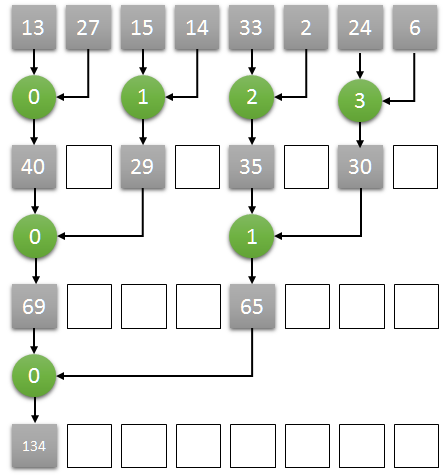
\includegraphics[scale=0.5]{imagenes/parallel_reduce.png}
\caption{Una reducción paralela de una sumatoria en CUDA.}
\label{image:cudareduction}
\end{figure}


En la figura \ref{image:cudareduction} podemos observar un ejemplo en el que se ve la estrucutra de cómo sería una reducción paralela en CUDA para un pequeño ejemplo. Para más información sobre cómo realizar una implementación de alto rendimiento de esta operación en CUDA puede consultarse en \cite{reduction}.\\

En nuestro trabajo la operación a la que queremos aplicar la reducción es el mínimo sobre un largo array de distancias. La operación mínimo \textbf{cumple la propiedad asociativa}, es decir:

$$min(min(a,b), c) = min(a, min(b, c))
$$

Además, si en vez pasar el valor para realizar la operación utilizamos un puntero en la memoria del dispositivo. Tras realizar toda la reducción con utilizar aritmética de punteros y restar al puntero inicial el puntero del valor mínimo obtenemos la solución deseada de forma eficiente. Una vez comprendido lo que esta operación implica, hemos decidido utilizar la función argmin de la librería CuPy que actúa de la forma comentada pero se encuentra altamente optimizada ofreciéndonos un gran rendimiento.

\begin{code}
\begin{minted}[fontsize=\footnotesize]{python}
import cupy as cp
min_index = cp.argmin(distances)
\end{minted}
\captionof{listing}{CuPy: Reducción para encontrar índice mínimo.\\}
\label{code:cupyreduce}
\end{code}


\subsubsection{Actualizar la BMU y su vecindario.}
Para esta operación necesitamos una vez tenemos encontrada la BMU actualizar una región alrededor de la misma y dependiente del parámetro de control $\sigma$, que controlaba el tamaño del vecindario. Recordemos que el parámetro $\sigma$ empezaba con un valor muy alto que se iba reduciendo exponencialmente y luego era fijado a otro parámetro indicado por el usuario, que debería de ser muy pequeño. Esto hace que en las primeras iteraciones se actualicen muchas neuronas y conforme vamos avanzando bastante menos. Los beneficios a la hora de paralelizar la actualización del mapa de neuronas de ese valor de $\sigma$, pues a mayor valor mayor es el número de neuronas alrededor que debemos evaluar. En esta implementación, hemos considerado siempre utilizar \textit{CUDA} para realizar la actualización pero sería una alternativa perfectamente viable utilizar la CPU en los casos en los que $\sigma$ es bajo y sólo un número pequeño de neuronas es afectado y el traslado de los datos necesarios de la matriz de pesos, que se encuentra en la GPU, de dispositivo a host y luego de vuelta no suponga un \textit{overhead} demasiado caro.\\

En la implementación que nosotros hemos realizado, que se corresponde a otro kernel de \textit{Numba} (código fuente \ref{code:updateonline}), cada hebra lanzada se corresponde a una neurona. Cada neurona comprueba su distancia con respecto a la BMU y si dicha distancia es válida procede a actualizar los datos que le corresponden conforme a la ecuación de actualización de pesos.

\begin{code}
\begin{minted}[fontsize=\footnotesize]{python}
@cuda.jit
def bmu_update(ids, samples, weights, d, bmu_row, 
    bmu_col, cols, eta, sigma_squared):
  idx = cuda.grid(1)
      if idx * d < weights.size:
          
          # 1. Medimos la distancia en la matriz del elemento actual a la BMU
          
          current_row = idx // cols
          current_col = idx % cols

          d_f = (current_col - bmu_col) * (current_col - bmu_col)
          d_f += (current_row - bmu_row) * (current_row - bmu_row)
          if d_f <= sigma_squared:
              # 2. Actualizamos acorde a esa distancia y el valor de sigma
              d_f = math.exp(-d_f/(2*sigma_squared))
              for i in range(d):
                  weights[idx * d + i] += eta * d_f * \
                  (samples[ids * d + i] - weights[idx * d + i])
\end{minted}
\captionof{listing}{Numba: Actualización de pesos de neuronas}
\label{code:updateonline}
\end{code}

\subsubsection{Actualizar los parámetros de control.}
Los parámetros de control $\eta$ y $\sigma$ son sólo dos parámetros a modificar por iteración y cuyo cálculo no es excesivamente complejo, razón por la que no es lo ideal paralelizar esta subproblema en la GPU y esto será realizando en la CPU, que, además puede realizar dicha operación de manera asíncrona mientras se está ejecutando alguno de los \textit{kernels}.

\subsubsection{Diagrama de flujo de la solución implementada.}
\begin{figure}[ht]
\centering
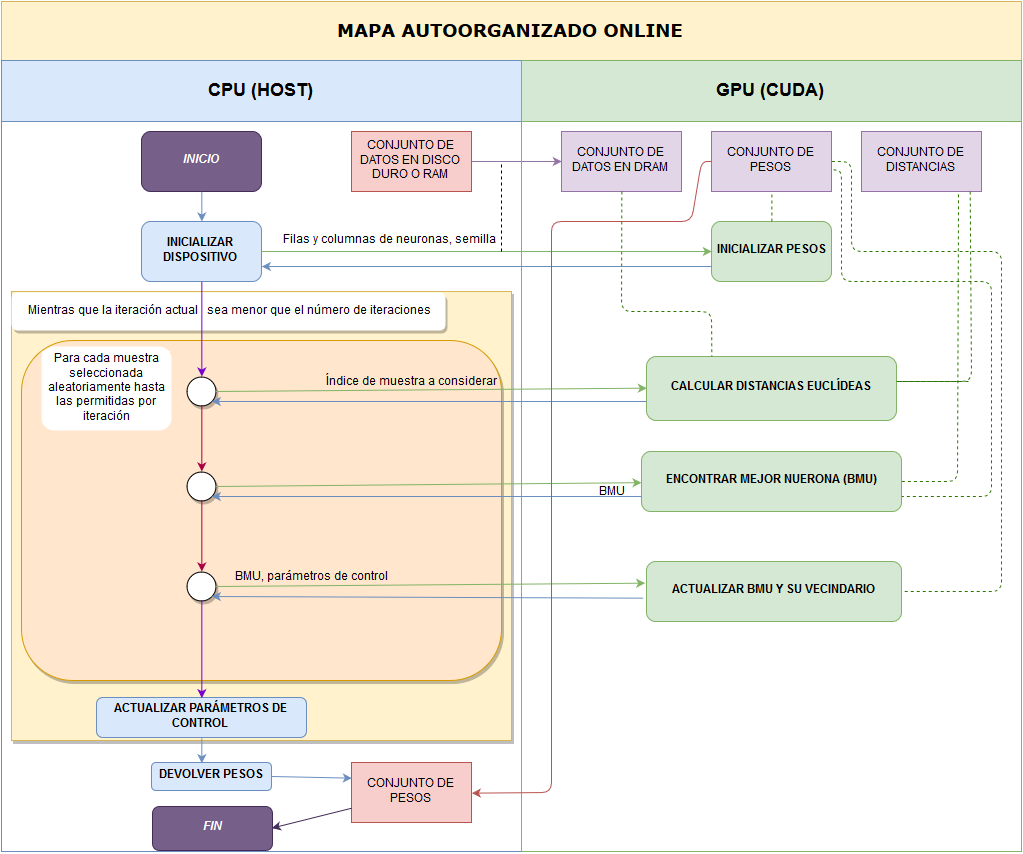
\includegraphics[scale=0.35]{imagenes/flujosomonline.png}
\caption{Diagrama de flujo para el mapa autoorganizado online.}
\end{figure}


\subsection{Desarrollo del mapa autoorganizado batch.}
En la versión \textit{batch} del algoritmo, aparece la posibilidad de evaluar múltiples muestras a la vez con el cambio de la ecuación de actualización de pesos. Ahora, en cada iteración los pesos de una neurona son la media de las muestras que lo activan y las que activan a las neuronas cercadas ponderada según la distancia en el vecindario del mapa. De manera similar a la sección anterior podemos subdividir el problema en pequeños subproblemas a resolver pero paralelizando en función del número de muestra en vez del de neuronas.

\begin{itemize}
  \item 1. Inicialización aleatoria de la matriz de pesos.
  \item 2. Cálculo de las distancias euclídeas entre todas las muestras y los pesos.
  \item 3. Encontrar la BMU para cada muestra.
  \item 4. Actualizar la matriz de pesos.
  \item 5. Actualizar los parámetros de control.
\end{itemize}

Tanto la \textbf{inicialización de la matriz de pesos} como la \textbf{actualización de los parámetros de control} son exáctamente \textbf{idénticas a la versión anterior} con ligeras variaciones, como que, por ejemplo, en la versión \textit{batch} no utilizamos la tasa de aprendizaje $\eta$ porque no es necesaria para obtener buenos resultados.\\

Para el \textbf{cálculo de las distancias euclídeas} necesitamos cambiar la idea planteada anteriormente puesto que ahora tenemos que evaluar todas las muestras con todas las neuronas. 
En este caso se lanzan tantas hebras como sea el producto del número de neuronas y el número de muestras, calculando cada hebra la distancia euclídea entre la muestra y la neurona que les corresponden. De manera similar a la anterior versión, obviamos el cálculo de la ráiz cuadrada. Puesto que ahora tenemos que evaluar todas las muestras a la vez no hemos planteado uso alguno de la memoria compartida para permitir que la solución sea aplicable a problemas de diversas características, pero si sabemos que la dimensión de una muestra del conjunto de datos no es excesivamente grande podríamos utilizar la memoria compartida para trabajar con los pesos del mapa. El código fuente \ref{code:euclideanbatch} muestra la implementación de este kernel en Numba.

\begin{code}
\begin{minted}[fontsize=\footnotesize]{python}
@cuda.jit
def batch_euclidean_distance(samples, weights, distances):
  idx = cuda.grid(1)
    if idx < distances.size:
        nrows, ncols, d = weights.shape
        nneurons = nrows * ncols
        row = idx // nneurons
        col = idx % nneurons
        wrow = col // ncols
        wcol = col % ncols

        my_distance = 0
        for i in range(d):
            i_distance = samples[row,i] - weights[wrow, wcol, i]
            my_distance += i_distance * i_distance
            
        distances[row, col] = my_distance
\end{minted}
\captionof{listing}{Numba: Distancia euclídea entre todas las muestras y neuronas.\\}
\label{code:euclideanbatch}
\end{code}

El proceso para \textbf{encontrar las BMU} vuelve a ser bastante similar utilizando la reducción. Sin embargo, ahora debemos de lanzar $N$ reducciones consecutivas para obtener la BMU de cada muestra. Utilizando CuPy podemos indicar si queremos hacer la reducción a lo largo de uno de los ejes, como se ve en el código fuente \ref{code:cupyreduce2}.

\begin{code}
\begin{minted}[fontsize=\footnotesize]{python}
import cupy as cp
# Se reduce cada fila
min_index = cp.argmin(distances, axis=1)
\end{minted}
\captionof{listing}{CuPy: Reducción para encontrar índice mínimo a lo largo de un eje en una matriz bidimensional.\\}
\label{code:cupyreduce2}
\end{code}

La parte más compleja de resolver en la versión \textit{batch} del algoritmo es la \textbf{actualización de la matriz de pesos}. Recordemos que en cada iteración, para obtener el nuevo vector de pesos hemos de aplicar la ecuación.

$$
 W_{i, j} = \frac{\sum_{k=0}^{f} \delta_f(c, [i,j]) \cdot X(T_k) }{\sum_{k=0}^{f} \delta_f(c, [i,j])}
$$\\

Por tanto, las neuronas que han sido activadas han de ser actualizadas en funcion de sus pesos. La solución que hemos planteado se basa en que primero se calculen las sumatorias del numerador y el denominador y posteriormente se pase otro kernel para hacer la división. Dado que al paralelizarlo existe la posibilidad de que múltiples hebras nos encontraríamos ante una condición de carrera lo que nos deja tres alternativas para resolver este problema.

\underline{Alternativas disponibles.}
\begin{itemize}
  \item a) Utilizar las operaciones de suma atómica del dispositivo.
  \item b) Utilizar una estructura auxiliar más grande y realizar reducciones sobre ella.
  \item c) Resolver este problema en la CPU.
\end{itemize}

La {opción a} fua la primera en ser implementada. El proceso se divide en dos \textit{kernels} uno que se encarga de generar los numeradores y denominadores para la fórmula de actualización nueva de cada neurona y otro que se encarga de hacer la división entre numerador y denominador para actualizar los pesos.\\

En el primero de estos \textit{kernels} (código fuente \ref{code:numbanumdem}) utilizamos la operación de suma atómica, esta operación es capaz de leer y escribir sobre una posición de memoria de la GPU en una única operación sin interferencia de ninguna otra hebra, lo que nos permite evitar el problema inicial limitando el rendimiento pero necesario para obtener resultados correctos. En la implementación propuesta, cada hebra se encargará de tomar la BMU de una muestra y actualizar su vecindario. 

\begin{code}
\begin{minted}[fontsize=\footnotesize]{python}
@cuda.jit
def prepare_update(bmu_row, bmu_col, samples, num, den, 
    nrows, ncols, sigma_squared):
  idx = cuda.grid(1)
    if idx < bmu_row.size:
        my_row = bmu_row[idx]
        my_col = bmu_col[idx]
        
        init_row = max(0, my_row - int(sigma_squared))
        finish_row = min(nrows, my_row + int(sigma_squared) + 1)
        
        init_col = max(0, my_col - int(sigma_squared))
        finish_col = min(ncols, my_col + int(sigma_squared) + 1)
        
    
        for i in range(init_row, finish_row):
            for j in range(init_col, finish_col):
                dist = (j-my_col) * (j-my_col) + (i-my_row) * (i-my_row)
    
                if dist <= sigma_squared:
                    hck = math.exp(-(dist)/(2 * sigma_squared))
                    cuda.atomic.add(den, i*ncols+j, hck)
                    d = samples.shape[1]
                    for k in range(d):
                        cuda.atomic.add(num, i*ncols*d + j*d +k,
                        hck * samples[idx, k])
\end{minted}
\captionof{listing}{Numba: Cálculo de numerador y denominador de la ecuación mediante suma atómica.\\}
\label{code:numbanumdem}
\end{code}

En el segundo kernel (código fuente \ref{code:numbaweightsbatch}), lanzamos tantas hebras como neuronas haya y actualizamos los pesos de cada neurona en función de los numeradores y denominadores calculados en el kernel anterior. Si esa neurona no se ha visto afectada en el cálculo de numeradores y denominadores, se mantiene los pesos de la iteración anterior.
\begin{code}
\begin{minted}[fontsize=\footnotesize]{python}
@cuda.jit
def finish_update(weights, num, den):
  idx = cuda.grid(1)
    if idx < den.size:
        nrows, ncols, d = weights.shape
        row = idx // ncols
        col = idx % ncols
        my_den = den[row * ncols + col]
        if my_den != 0:
            for k in range(d):
                weights[row, col, k] = num[row*ncols*d + col*d +k] / my_den
      
        cuda.syncthreads()
       
        for k in range(d):
            num[row*ncols*d + col*d +k] = 0
            
        den[row * ncols + col] = 0
\end{minted}
\captionof{listing}{Numba: Actualización de pesos en función de numeradores y denominadores.\\}
\label{code:numbaweightsbatch}
\end{code}


El procedimiento será mucho más costoso en las primeras iteraciones y menos costoso conforme se avance al irse reduciendo el vecindario. Para evaluar el rendimiento de esta versión utilizamos el profiler de NVIDIA, \textbf{nvprof} para medir el tiempo que se tarda en obtener los resultados de esta forma así como el tiempo que ha tardado en ejecutarse el algoritmo. Para realizar el profile hemos utilizado el conjunto de datos de las caras de \textit{Olivetti} (explicado en el siguiente capítulo). En la tabla \ref{tab:batchprofileparams} podemos observar los parámetros de control utilizados para la ejecución de este ejemplo.

\begin{table}[ht]
\begin{tabular}{|l|l|l|l|l|l|l|l|}
\hline
\multicolumn{1}{|c|}{\textbf{Muestras}} & \textbf{Dimensión} & \multicolumn{1}{c|}{\textbf{Neuronas}} & \textbf{Épocas} & \textbf{\begin{tabular}[c]{@{}l@{}}Épocas\\ 1º Fase\end{tabular}} & $\sigma_0$ & $\sigma_f$ & $\tau$ \\ \hline
400                                     & 4096               & 400 (20x20)                            & 400             & 100                                                               & 15         & 0.1        & 400    \\ \hline
\end{tabular}
\caption{Parámetros de control para el ejemplo utilizando en el profiler.}
\label{tab:batchprofileparams}
\end{table}


Los resultados más relevantes proporcionados por el profiler se encuentran en la tabla \ref{tab:batchprofile}.\\

\begin{table}[ht]
\centering
\begin{tabular}{|l|l|crrr}
\hline
\rowcolor[HTML]{EFEFEF} 
\multicolumn{1}{|c|}{\cellcolor[HTML]{EFEFEF}\textbf{Actividad}}                                                  & \multicolumn{1}{c|}{\cellcolor[HTML]{EFEFEF}\textbf{\begin{tabular}[c]{@{}c@{}}Tiempo\\ total\end{tabular}}} & \multicolumn{1}{c|}{\cellcolor[HTML]{EFEFEF}\textbf{\begin{tabular}[c]{@{}c@{}}Nº\\usos\end{tabular}}} & \multicolumn{1}{c|}{\cellcolor[HTML]{EFEFEF}\textbf{\begin{tabular}[c]{@{}c@{}}Mín\end{tabular}}} & \multicolumn{1}{c|}{\cellcolor[HTML]{EFEFEF}\textbf{\begin{tabular}[c]{@{}c@{}}Medio\end{tabular}}} & \multicolumn{1}{c|}{\cellcolor[HTML]{EFEFEF}\textbf{\begin{tabular}[c]{@{}c@{}}Máx\end{tabular}}} \\ \hline
\rowcolor[HTML]{EFEFEF} 
\cellcolor[HTML]{F8A102}\textbf{CPU + GPU}                                                                        & \cellcolor[HTML]{F8A102}56,62 s                                                                              & \multicolumn{1}{l}{\cellcolor[HTML]{EFEFEF}}                                                               & \multicolumn{1}{l}{\cellcolor[HTML]{EFEFEF}}                                                                  & \multicolumn{1}{l}{\cellcolor[HTML]{EFEFEF}}                                                                  & \multicolumn{1}{l}{\cellcolor[HTML]{EFEFEF}}                                                                  \\ \cline{1-2}
\rowcolor[HTML]{EFEFEF} 
\cellcolor[HTML]{38FFF8}\textbf{GPU}                                                                              & \cellcolor[HTML]{38FFF8}55,37 {[}100 \%{]}                                                                   & \multicolumn{1}{l}{\cellcolor[HTML]{EFEFEF}}                                                               & \multicolumn{1}{l}{\cellcolor[HTML]{EFEFEF}}                                                                  & \multicolumn{1}{l}{\cellcolor[HTML]{EFEFEF}}                                                                  & \multicolumn{1}{l}{\cellcolor[HTML]{EFEFEF}}                                                                  \\ \hline
\rowcolor[HTML]{ECF4FF} 
\textbf{\begin{tabular}[c]{@{}l@{}}Cálculo de\\ distancias\end{tabular}}                                          & 14,67 s {[}26,5 \%{]}                                                                                        & \multicolumn{1}{c|}{\cellcolor[HTML]{ECF4FF}400}                                                           & \multicolumn{1}{r|}{\cellcolor[HTML]{ECF4FF}35,67 ms}                                                         & \multicolumn{1}{r|}{\cellcolor[HTML]{ECF4FF}35,68 ms}                                                         & \multicolumn{1}{r|}{\cellcolor[HTML]{ECF4FF}45,58 ms}                                                         \\ \hline
\rowcolor[HTML]{ECF4FF} 
\textbf{\begin{tabular}[c]{@{}l@{}}Encontrar \\ BMUs\end{tabular}}                                                & 23,78 ms {[}0,04 \%{]}                                                                                       & \multicolumn{1}{c|}{\cellcolor[HTML]{ECF4FF}400}                                                           & \multicolumn{1}{r|}{\cellcolor[HTML]{ECF4FF}54,82 $\mu$s}                                                     & \multicolumn{1}{r|}{\cellcolor[HTML]{ECF4FF}59,47 $\mu$s}                                                     & \multicolumn{1}{r|}{\cellcolor[HTML]{ECF4FF}68,26 $\mu$s}                                                     \\ \hline
\rowcolor[HTML]{ECF4FF} 
{\color[HTML]{CB0000} \textbf{\begin{tabular}[c]{@{}l@{}}Generar \\ numeradores y \\ denominadores\end{tabular}}} & {\color[HTML]{FE0000} \textbf{39,97 s {[}72,19 \%{]}}}                                                       & \multicolumn{1}{c|}{\cellcolor[HTML]{ECF4FF}400}                                                           & \multicolumn{1}{r|}{\cellcolor[HTML]{ECF4FF}1,05 ms}                                                          & \multicolumn{1}{r|}{\cellcolor[HTML]{ECF4FF}99,93 ms}                                                         & \multicolumn{1}{r|}{\cellcolor[HTML]{ECF4FF}458,2 ms}                                                         \\ \hline
\rowcolor[HTML]{ECF4FF} 
\textbf{\begin{tabular}[c]{@{}l@{}}Actualizar \\matriz  de pesos\end{tabular}}                                    & 695,01 ms {[}1,26 \%{]}                                                                                      & \multicolumn{1}{c|}{\cellcolor[HTML]{ECF4FF}400}                                                           & \multicolumn{1}{r|}{\cellcolor[HTML]{ECF4FF}1,68 ms}                                                          & \multicolumn{1}{r|}{\cellcolor[HTML]{ECF4FF}1,74 ms}                                                          & \multicolumn{1}{r|}{\cellcolor[HTML]{ECF4FF}1,86 ms}                                                          \\ \hline
\end{tabular}
\caption{Resumen de tiempos más importantes de la ejecución del profiler.}
\label{tab:batchprofile}
\end{table}

Podemos observar que el cuello de botella en esta ejecución es el kernel asociado a computar los numeradores y denominadores, ocupando el 72 \% del tiempo de ejecución de la CPU. Por ello, vamos a analizar el resto de opciones para ver cuál es su rendimiento.

La \textbf{opción b} fue descartada pues conllevaría serían necesarias dos estructuras auxiliares para almacenar los numeradores y los denominadores. En el caso en cuestión, necesitaríamos 2,5 GiB para los numeradores y 625 KiB que generan una complejidad espacial excesiva.\\

Dados los resultados de la opción a, hemos decidido probar también a implementar la \textbf{opción c}. En esta versión, el cálculos de distancias y encontrar la BMU es realizado en la GPU y la actualización de pesos en la CPU con el fin de evaluar si el gran porcentaje de tiempo que se tarda es por la dificultad del problema o porque las operaciones atómicas del dispostivo \textit{CUDA} no son lo suficientemente eficientes. Tras evaluarlo empíricamente, el tiempo total de ejecución de esta opción alcanzó los 160,56 segundos que es mucho más lento que los 56,62 segundos de la opción a. Por tanto, esta opción también fue descartada y nos quedamos con la implementación inicial utilizando la suma atómica.


\subsubsection{Diagrama de flujo de la solución final implementada.}

\begin{figure}[ht]
\centering
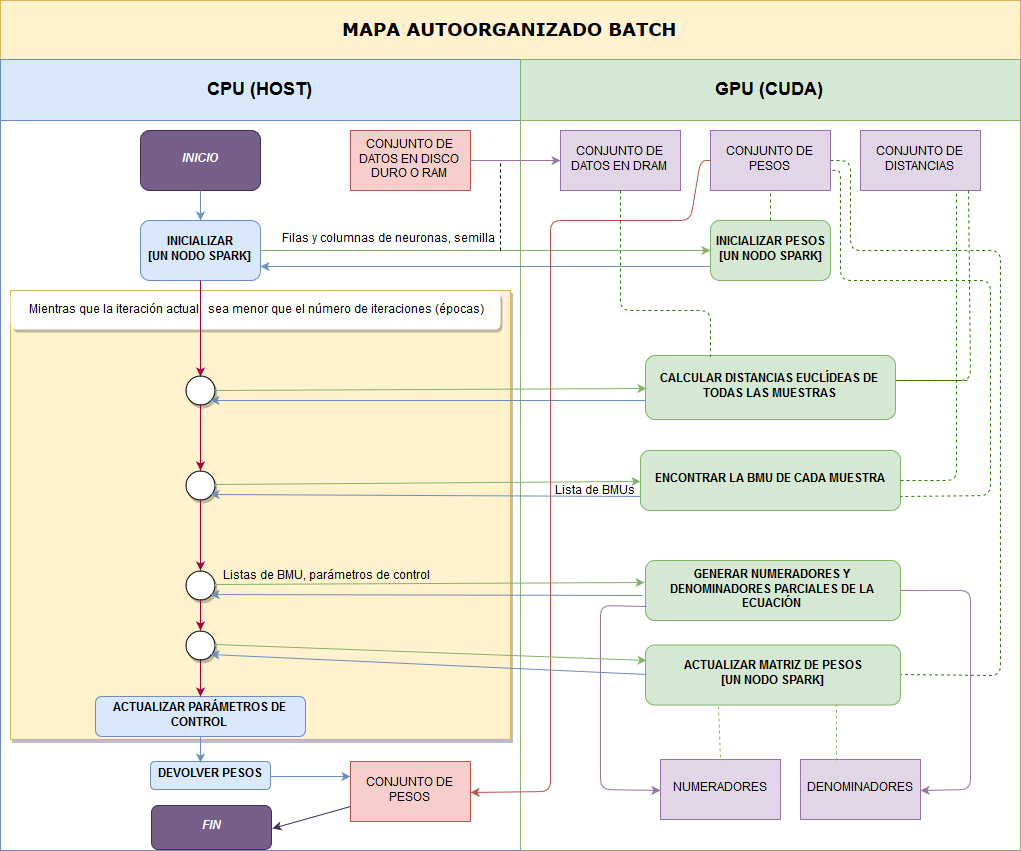
\includegraphics[scale=0.35]{imagenes/flujosombatch.png}
\caption{Diagrama de flujo para el mapa autoorganizado batch.}
\end{figure}